\documentclass{article}
\iffalse
This file is protected by Copyright. Please refer to the COPYRIGHT file
distributed with this source distribution.

This file is part of OpenCPI <http://www.opencpi.org>

OpenCPI is free software: you can redistribute it and/or modify it under the
terms of the GNU Lesser General Public License as published by the Free Software
Foundation, either version 3 of the License, or (at your option) any later
version.

OpenCPI is distributed in the hope that it will be useful, but WITHOUT ANY
WARRANTY; without even the implied warranty of MERCHANTABILITY or FITNESS FOR A
PARTICULAR PURPOSE. See the GNU Lesser General Public License for more details.

You should have received a copy of the GNU Lesser General Public License along
with this program. If not, see <http://www.gnu.org/licenses/>.
\fi

\author{} % Force author to be blank
%----------------------------------------------------------------------------------------
% Paper size, orientation and margins
%----------------------------------------------------------------------------------------
\usepackage{geometry}
\geometry{
	letterpaper,			% paper type
	portrait,				% text direction
	left=.75in,				% left margin
	top=.75in,				% top margin
	right=.75in,			% right margin
	bottom=.75in			% bottom margin
 }
%----------------------------------------------------------------------------------------
% Header/Footer
%----------------------------------------------------------------------------------------
\usepackage{fancyhdr} \pagestyle{fancy} % required for fancy headers
\renewcommand{\headrulewidth}{0.5pt}
\renewcommand{\footrulewidth}{0.5pt}
\rhead{\small{ANGRYVIPER Team}}
%----------------------------------------------------------------------------------------
% Appendix packages
%----------------------------------------------------------------------------------------
\usepackage[toc,page]{appendix}
%----------------------------------------------------------------------------------------
% Defined Commands & Renamed Commands
%----------------------------------------------------------------------------------------
\renewcommand{\contentsname}{Table of Contents}
\renewcommand{\listfigurename}{List of Figures}
\renewcommand{\listtablename}{List of Tables}
\newcommand{\todo}[1]{\textcolor{red}{TODO: #1}\PackageWarning{TODO:}{#1}} % To do notes
\newcommand{\code}[1]{\texttt{#1}} % For inline code snippet or command line
%----------------------------------------------------------------------------------------
% Various pacakges
%----------------------------------------------------------------------------------------
\usepackage{hyperref} % for linking urls and lists
\usepackage{graphicx} % for including pictures by file
\usepackage{listings} % for coding language styles
\usepackage{rotating} % for sideways table
\usepackage{pifont}   % for sideways table
\usepackage{pdflscape} % for landscape view
%----------------------------------------------------------------------------------------
% Table packages
%----------------------------------------------------------------------------------------
\usepackage{tabularx} % c=center,l=left,r=right,X=fill
\usepackage{float}
\floatstyle{plaintop}
\usepackage[tableposition=top]{caption}
\newcolumntype{P}[1]{>{\centering\arraybackslash}p{#1}}
\newcolumntype{M}[1]{>{\centering\arraybackslash}m{#1}}
%----------------------------------------------------------------------------------------
% Block Diagram / FSM Drawings
%----------------------------------------------------------------------------------------
\usepackage{tikz}
\usetikzlibrary{shapes,arrows,fit,positioning}
\usetikzlibrary{automata} % used for the fsm
%----------------------------------------------------------------------------------------
% Colors Used
%----------------------------------------------------------------------------------------
\usepackage{colortbl}
\definecolor{blue}{rgb}{.7,.8,.9}
\definecolor{ceruleanblue}{rgb}{0.16, 0.32, 0.75}
\definecolor{drkgreen}{rgb}{0,0.6,0}
\definecolor{deepmagenta}{rgb}{0.8, 0.0, 0.8}
\definecolor{cyan}{rgb}{0.0,0.6,0.6}
\definecolor{maroon}{rgb}{0.5,0,0}
%----------------------------------------------------------------------------------------
% Update the docTitle and docVersion per document
%----------------------------------------------------------------------------------------
\def\docTitle{Component Data Sheet}
\def\docVersion{1.3}
%----------------------------------------------------------------------------------------
\date{Version \docVersion} % Force date to be blank and override date with version
\title{\docTitle}
\lhead{\small{\docTitle}}

\def\comp{lime\_rx\_proxy}
\edef\ecomp{lime_rx_proxy}
\def\Comp{Lime RX Proxy}
\graphicspath{ {figures/} }

\begin{document}

\section*{Summary - \Comp}
\begin{tabular}{|c|M{13.5cm}|}
	\hline
	\rowcolor{blue}
	                  &                \\
	\hline
	Name              & \comp          \\
	\hline
	Worker Type       & Proxy          \\
	\hline
	Version           & v\docVersion \\
	\hline
	Release Date      & February 2018 \\
	\hline
	Component Library & ocpi.assets.devices   \\
	\hline
	Workers           & \comp.rcc      \\
	\hline
	Tested Platforms  & linux-x13\_3-arm, CentOS 7 (via ALST4/Zipper), CentOS 6/7 (via ML605/Zipper for HPC and LPC FMC slots) \\
	\hline
	Slave Worker      & lime\_rx.hdl   \\
	\hline
\end{tabular}

\section*{Functionality}
This control proxy is designed to allow the user of the proxy to set more user friendly properties than the register map on the LMS6002D Transceiver.  Only the control of the RX portion of the LMS6002D Transceiver is encompassed in this worker.

\section*{Worker Implementation Details}
\subsection*{\comp.rcc}
A diagram of the receiver in the Lime Microsystems LMS6002D can be seen in Figure \ref{fig:hw}. It consists of a single channel with three separate inputs each with a dedicated LNA. Post LNA, the RF signal is then mixed with a PLL output to directly down convert to baseband. Post mixing, there an programmable gain amplifier, a lowpass filter, and an another programmable gain amplifier. Furthermore, DC offset is applied at the input of the second programmable gain amplifier. The resulting analog receive IQ signals are converted into the digital domain using the on chip ADCs and are provided as an output.\par\medskip
\noindent The features described above are controllable via a SPI interface on the LMS6002D. This proxy is responsible for translating its properties (as described in the Lime datasheet) into the required SPI reads and writes and controlling the worker which performs the SPI transactions.
\newpage

\section*{Block Diagrams}
\subsection*{Top level}
\begin{figure}[ht]
	\centerline{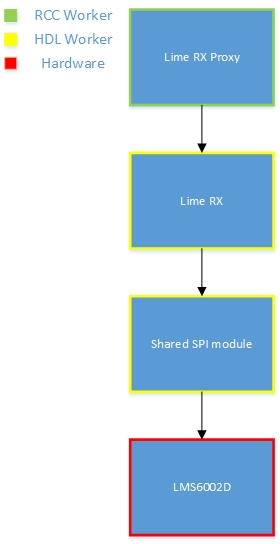
\includegraphics[scale=0.7]{lime_RX_toplevel}}
	\caption{Top Level Block Diagram}
	\label{fig:top}
\end{figure}
\vspace{25 mm}

\subsection*{Hardware}
\begin{figure}[ht]
	\centerline{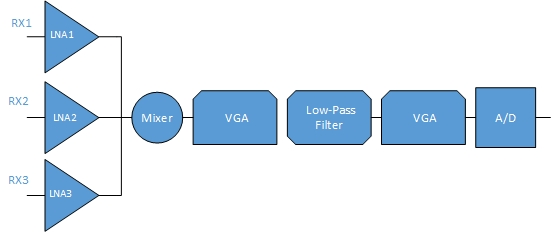
\includegraphics[scale=0.7]{lime_RX_HW}}
	\caption{Hardware Block Diagram}
	\label{fig:hw}
\end{figure}
\vspace{25 mm}

\section*{Source Dependencies}
\begin{itemize}
	\item ocpi.assets/hdl/devices/lime\_rx\_proxy.rcc/lime\_rx\_proxy.cc
	\item ocpi.assets/hdl/devices/lime\_rx\_proxy.rcc/lime\_shared.h
\end{itemize}

\begin{landscape}
	\section*{Component Spec Properties}
	\begin{scriptsize}
		\begin{tabular}{|p{3cm}|c|c|c|c|c|c|p{10cm}|}
			\hline
			\rowcolor{blue}
			Name                          & Type   & Sequence & Array      & Accessibility       & Valid & Default & Usage                                                                                                                                                                                                                                                              \\
			\rowcolor{blue}
			                              &        & Length   & Dimensions &                     & Range &         &                                                                                                                                                                                                                                                                    \\
			\hline
			\verb+ninputs+                & UChar  & -        & -          & Readable, Parameter & 1-3   & 1       & The number of hardware inputs that are available to this RX.                                                                                                                                                                                                       \\
			\hline
			\verb+input_select+           & UChar  & -        & -          & Writable, Readable  & -     & -       & This is the hardware selection of which input to pass to the mixer. Input 1 rated from 300MHz to 2.8GHz, input 2 rated from 1.5GHz to 3.8GHz, and input 3 rated from 300MHz to 3GHz.                                                                               \\
			\hline
			\verb+input_gain_db+          & Short  & -        & -          & Writable, Readable  & -     & -       & The gain value in the input LNA.                                                                                                                                                                                                                                   \\
			\hline
			\verb+center_freq_hz+         & Double & -        & -          & Writable, Readable  & -     & -       & The value of the tuned center frequency of the receiver.                                                                                                                                                                                                           \\
			\hline
			\verb+post_mixer_dc_offset_i+ & UChar  & -        & -          & Writable, Readable  & -     & -       & The register value used to tune the DC offset of the received signal to close to zero on the I path. This is generally set to a close value and then a VHDL component is used to tun this to be exact. The mapping of this is described in the Lime documentation. \\
			\hline
			\verb+post_mixer_dc_offset_q+ & UChar  & -        & -          & Writable, Readable  & -     & -       & The register value used to tune the DC offset of the received signal to close to zero on the Q path. This is generally set to a close value and then a VHDL component is used to tun this to be exact. The mapping of this is described in the Lime documentation. \\
			\hline
			\verb+pre_lpf_gain_db+        & Short  & -        & -          & Writable, Readable  & -     & -       & The gain value for the VGA in before the low pass filter.                                                                                                                                                                                                          \\
			\hline
			\verb+lpf_bw_hz+              & Float  & -        & -          & Writable, Readable  & -     & -       & The low pass filter that is used to filter out any noise on the received signal.                                                                                                                                                                                   \\
			\hline
			\verb+post_lpf_gain_db+       & Short  & -        & -          & Writable, Readable  & -     & -       & The gain value for the VGA in after the low pass filter. The value is in dB and can only be set in multiples of 3.                                                                                                                                                 \\
			\hline
		\end{tabular}
	\end{scriptsize}

	\section*{Worker Properties}
	\subsection*{\comp.rcc}
	\begin{scriptsize}
		\begin{tabular}{|p{2cm}|p{3cm}|c|c|c|c|p{2.5cm}|c|p{7cm}|}
			\hline
			\rowcolor{blue}
			Type         & Name                          & Type & Sequence & Array      & Accessibility/ & Valid Range                                                                                                    & Default & Usage                                                                                                                                                                                                                                                               \\
			\rowcolor{blue}
			             &                               &      & Length   & Dimensions & Advanced       &                                                                                                                &         &                                                                                                                                                                                                                                                                     \\
			\hline
			SpecProperty & \verb+ninputs+                & -    & -        & -          & -              & 3                                                                                                              & 3       & The number of hardware inputs that are available to this RX.                                                                                                                                                                                                        \\
			\hline
			SpecProperty & \verb+input_select+           & -    & -        & -          & WriteSync      & 1-3                                                                                                            & -       & This is the hardware selection of which input to pass to the mixer. Input 1 rated from 300MHz to 2.8GHz, input 2 rated from 1.5GHz to 3.8GHz, and input 3 rated from 300MHz to 3GHz.                                                                                \\
			\hline
			SpecProperty & \verb+input_gain_db+          & -    & -        & -          & WriteSync      & -6,0,6                                                                                                         & -       & The gain value in the input LNA.                                                                                                                                                                                                                                    \\
			\hline
			SpecProperty & \verb+center_freq_hz+         & -    & -        & -          & WriteSync      & 232,500 - 3,720,000                                                                                            & -       & The value of the tuned center frequency of the receiver.                                                                                                                                                                                                            \\
			\hline
			SpecProperty & \verb+post_mixer_dc_offset_i+ & -    & -        & -          & WriteSync      & 0x00-0x80                                                                                                      & -       & The register value used to tune the DC offset of the received signal to close to zero on the I path. This is generally set to a close value and then a VHDL component is used to tun this to be exact. The mapping of this is described in the Lime documentation.  \\
			\hline
			SpecProperty & \verb+post_mixer_dc_offset_q+ & -    & -        & -          & WriteSync      & 0x00-0x80                                                                                                      & -       & TThe register value used to tune the DC offset of the received signal to close to zero on the Q path. This is generally set to a close value and then a VHDL component is used to tun this to be exact. The mapping of this is described in the Lime documentation. \\
			\hline
			SpecProperty & \verb+pre_lpf_gain_db+        & -    & -        & -          & WriteSync      & 5,19,30                                                                                                        & -       & TThe gain value for the VGA in before the low pass filter.                                                                                                                                                                                                          \\
			\hline
			SpecProperty & \verb+lpf_bw_hz+              & -    & -        & -          & WriteSync      & 14e6, 10e6, 7e6, 6e6, 5e6, 4.375e6, 3.5e6, 3e6, 2.75e6, 2.5e6, 1.92e6, 1.5e6, 1.375e6, 1.25e6, 0.875e6, 0.75e6 & -       & The low pass filter that is used to filter out any noise on the received signal.                                                                                                                                                                                    \\
			\hline
			SpecProperty & \verb+post_lpf_gain_db+       & -    & -        & -          & WriteSync      & 0 to 30                                                                                                        & -       & The gain value for the VGA in after the low pass filter. The value is in dB and can only be set in multiples of 3.                                                                                                                                                  \\
			\hline
		\end{tabular}
	\end{scriptsize}
\end{landscape}

\section*{Performance and Resource Utilization}
\subsubsection*{\comp.rcc}
\begin{scriptsize}
	\begin{tabular}{|c|c|c|}
		\hline
		\rowcolor{blue}
		Processor Type & Processor Frequency & Run Function Time \\
		\hline
		TBD            & TBD                 & TBD               \\
		\hline
	\end{tabular}
\end{scriptsize}

\section*{Test and Verification}
The testbench for this proxy is meant to exercise the properties of the proxy worker dynamically while the application is running. The sample rate is set low and not changed so that there is less data to deal with at the end. The test requires that there be a signal generator capable of generating a sine wave from 300MHz to 3.005GHz connected to the RX interface of the radio. Amplitude levels are suggested below, but if the test yields all zeros for the I/Q values when plotted, consider increasing the signal generator gain. Also, note that the once the test is started, data is being written to file continuously, so completing the test quickly helps with data consistency.\par\medskip
\noindent The following steps are taken in the testbench:
\begin{enumerate}
	\item Toggle the input select (only when Matchstiq-Z1 container is detected/being used)
	\item Change the input gain settings
	\item Change pre-lpf gain settings
	\item Change filter values
	\item Tune the center frequency
\end{enumerate}
\newpage
\subsection*{Matchstiq-Z1}
For Matchstiq-Z1 testing, the sample rate is set at 100 kS/s. The signal generator amplitude should be set to -55 dBm.
The results should look like the below images:
\begin{figure}[ht]
	\centerline{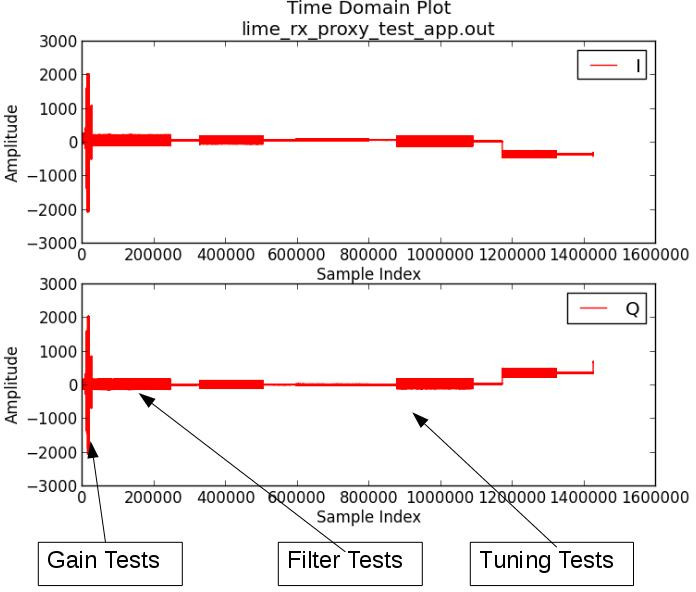
\includegraphics[scale=0.5]{lime_RX_big_testbench}}
	\caption{Full Testbench}
\end{figure}
\begin{figure}[ht]
	\centerline{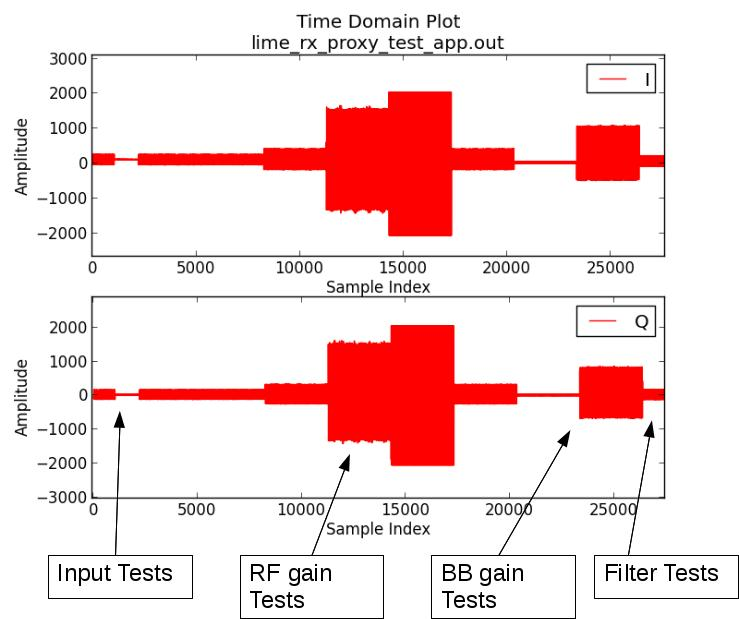
\includegraphics[scale=0.5]{lime_RX_small_testbench}}
	\caption{Refined Gain Testing Stage}
\end{figure}
\newpage
\subsection*{Zipper Platforms}
For Zipper Platform testing, the sample rate is set at 500 kS/s. The signal generator amplitude should be set to -30 dBm. The results should look like the below images:
\begin{figure}[h]
	\centerline{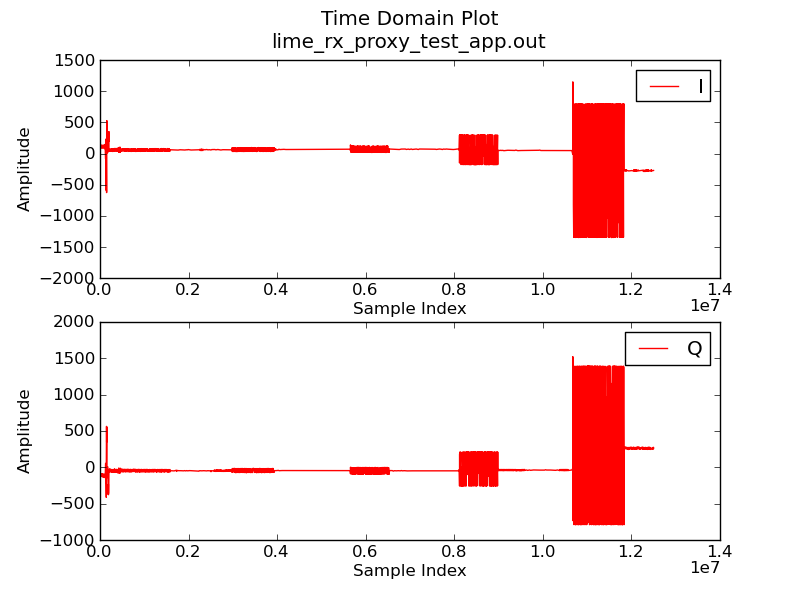
\includegraphics[scale=0.5]{zedboard_output_large}}
	\caption{Full Testbench}
\end{figure}
\begin{figure}[h]
	\centerline{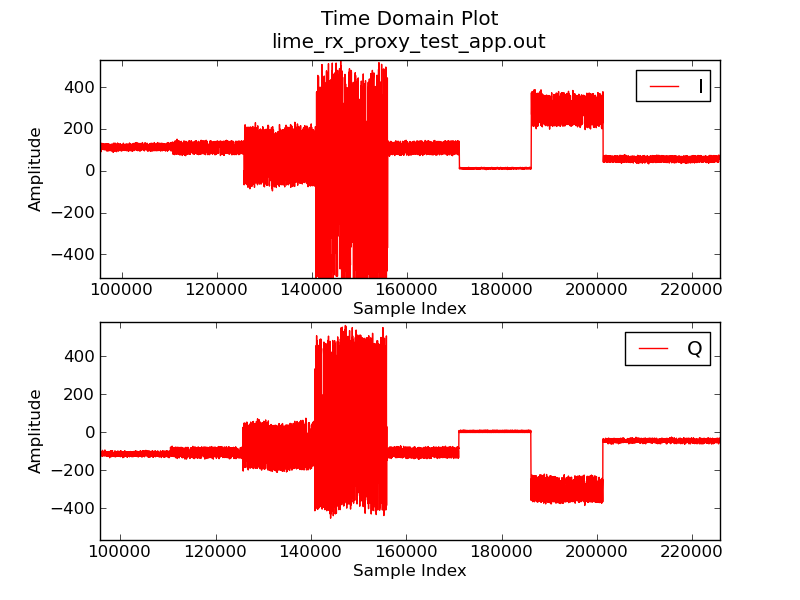
\includegraphics[scale=0.5]{zedboard_output_small}}
	\caption{Refined Gain Testing Stage}
\end{figure}
\section*{References}
\begin{flushleft}
	\begin{itemize}
		\item[1)] LMS6002D Datasheet, www.limemicro.com
	\end{itemize}
\end{flushleft}
\end{document}
